\begin{figure}[!htb]
\centering
\noindent\makebox[\linewidth][c]{%
  \setlength{\unitlength}{1mm}%
  \begin{picture}(185,181)
    \put(0,0){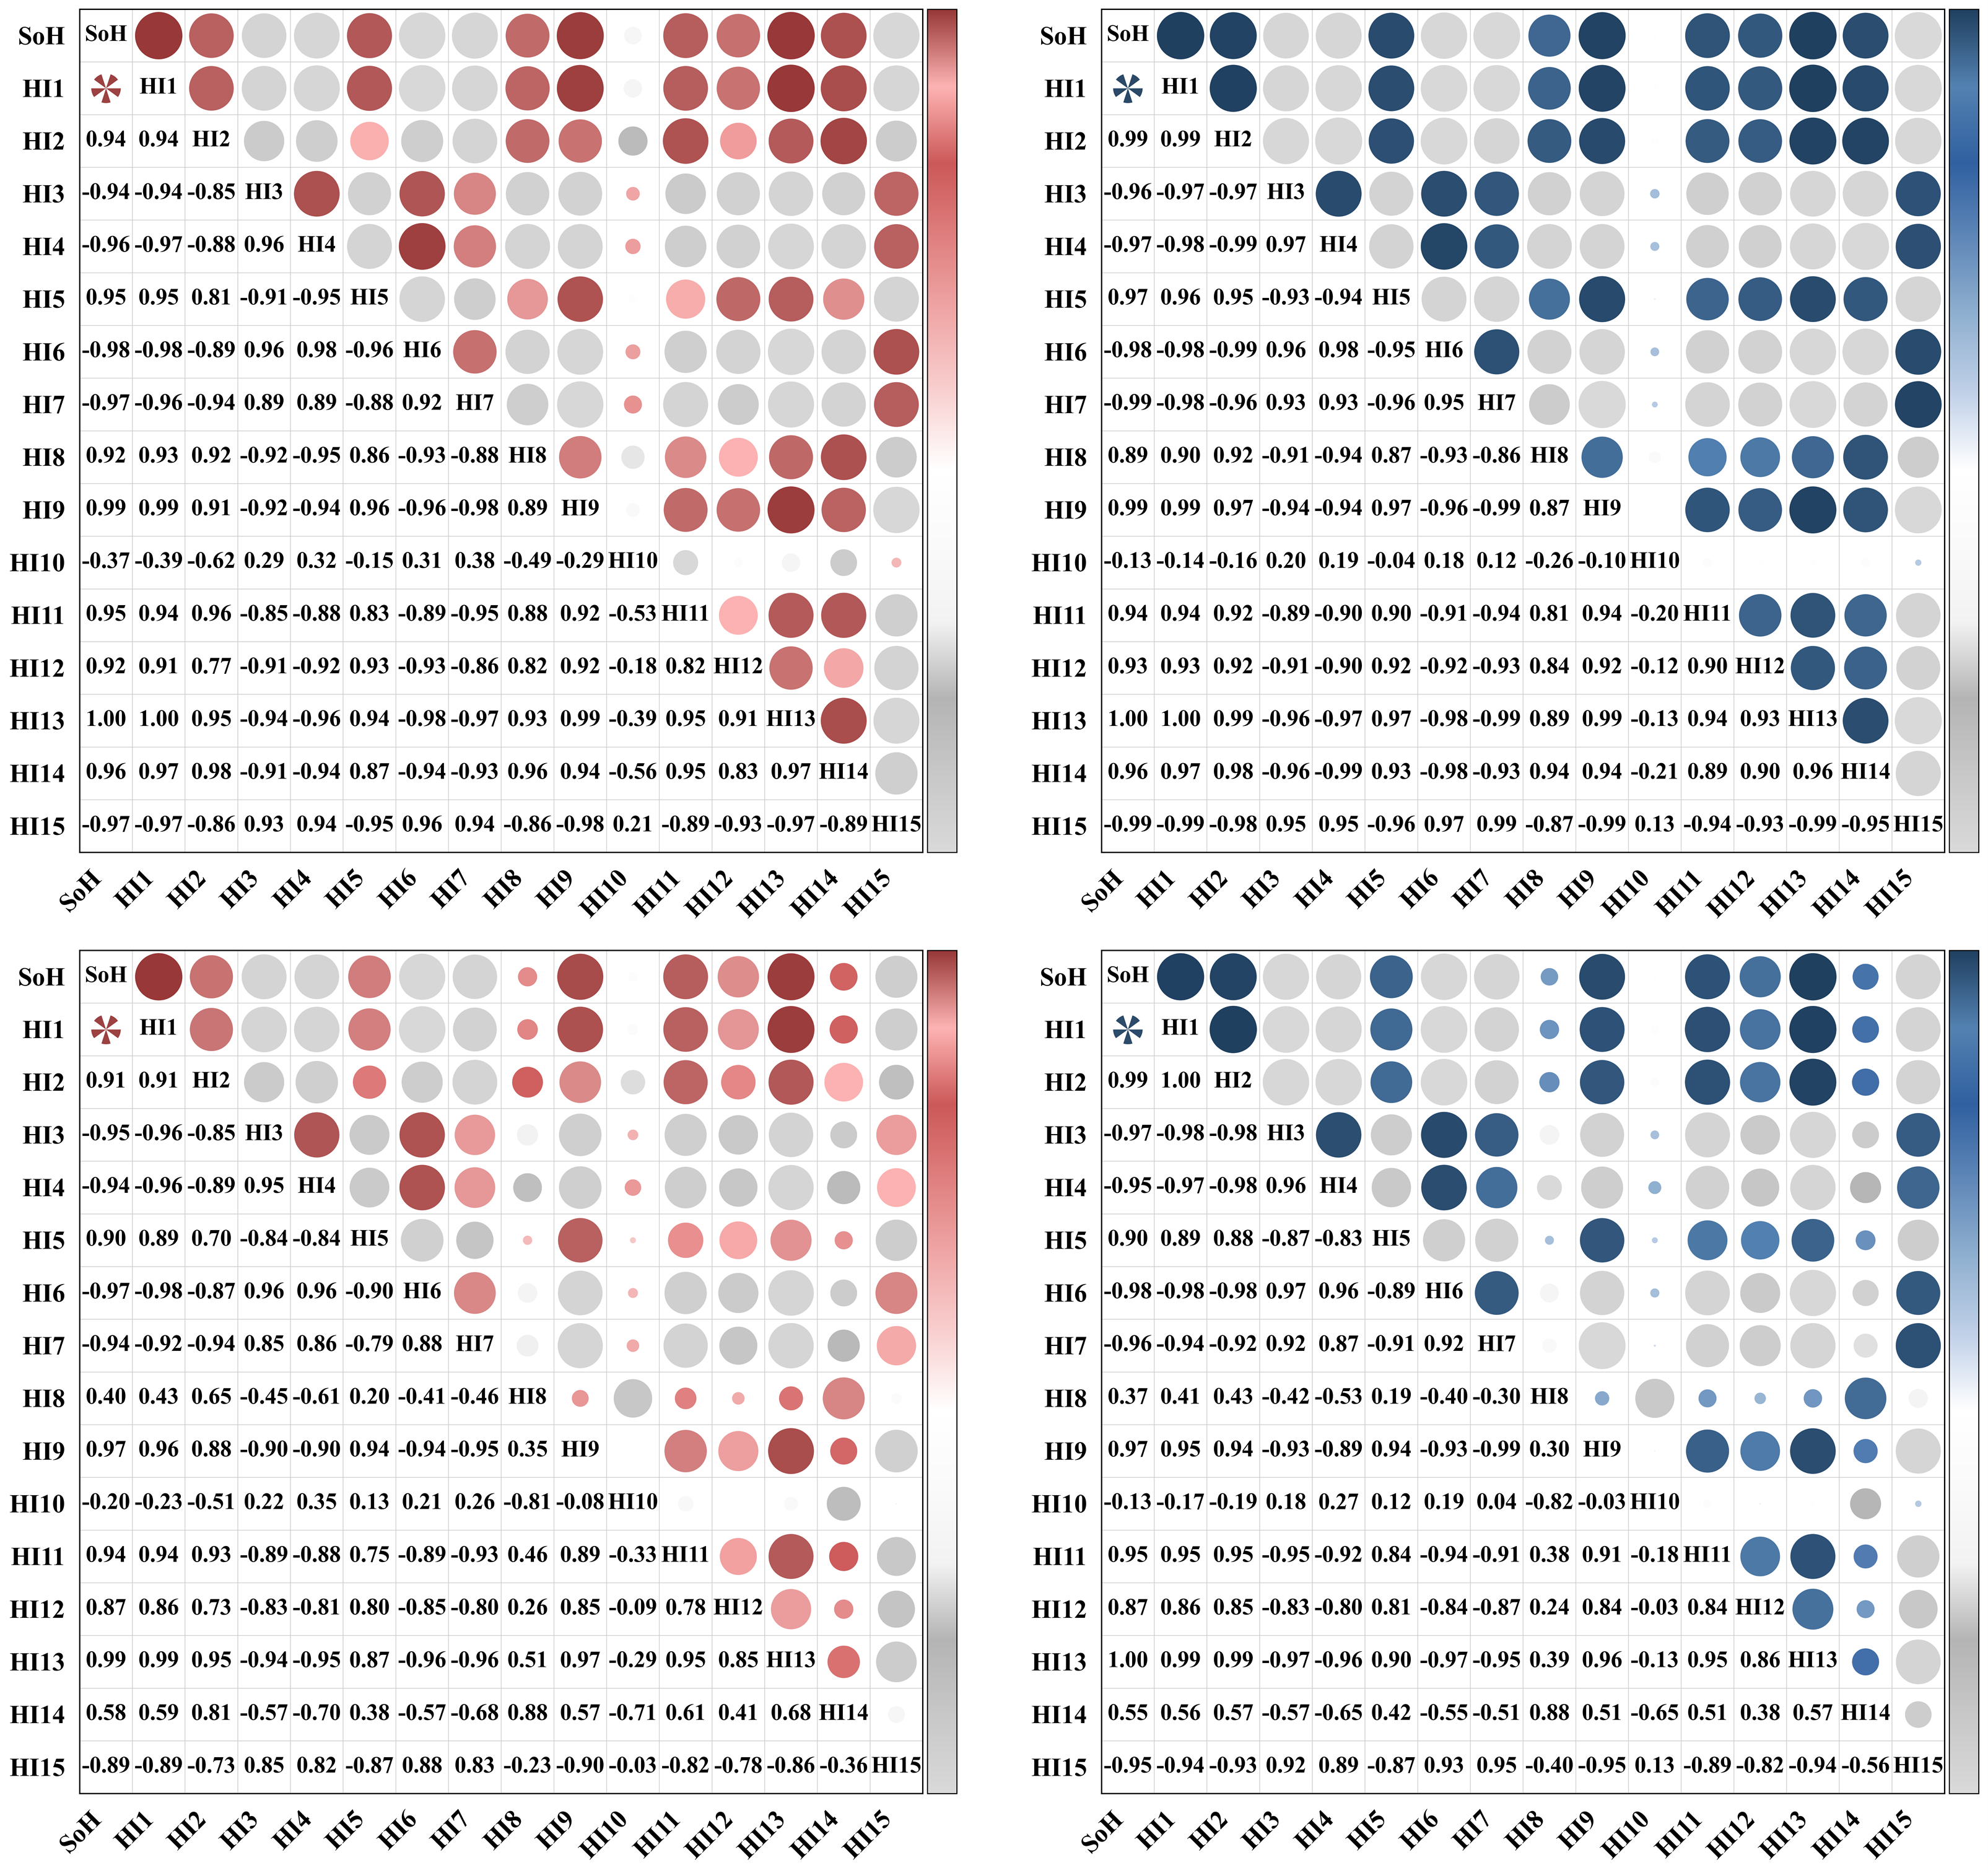
\includegraphics[width=185mm]{figures/fig4_pccscc_print.png}}
    \put(0,177){\makebox(0,0)[l]{\small (a)}}
    \put(98,177){\makebox(0,0)[l]{\small (b)}}
    \put(0,87){\makebox(0,0)[l]{\small (c)}}
    \put(98,87){\makebox(0,0)[l]{\small (d)}}
  \end{picture}%
}
\caption{Correlation matrices of candidate HIs and SOH on the Oxford dataset: (a) Cell1, PCC; (b) Cell1, SCC; (c) Cell2, PCC; (d) Cell2, SCC.}
\label{fig:2-4}
\end{figure}
